

\chapter{Litt om inkludering av MATLAB-kode}\label{kap:kode}


\section{Pakkene \fbox{\tt listings} og \fbox{\tt mcode}}\label{delkap:lstinput}
Ved å legge til pakken \fbox{\tt listings} 
kan du enkelt inkludere all slags kode i {\LaTeX}. Pakken \fbox{\tt mcode}
er en tilleggspakke som tilpasser {\tt listings} til å presentere MATLAB-kode.

Du kan typisk bruke {\tt listings} på 2 måter som vist i de neste delkapitlene.

\subsection{Dynamisk med \fbox{\tt  $\backslash$lstinputlisting}-kommandoen}
Ved å  
bruke \fbox{\tt  $\backslash$lstinputlisting}-kommandoen oppretter du 
en dynamisk link til selve fila du ønsker å inkludere i rapporten.
Fordelen med å inkludere kode på denne måten 
er at dersom du oppdaterer MATLAB-fila, vil
rapporten oppdateres automatisk neste gang du kompilerer {\LaTeX}-dokumentet.

\newpage
Et eksempel på hvor slik kode er brukt er i
kodeutdrag~\ref{kode:SaveMyFigure}, hvor {\LaTeX}-koden 
ser slik ut:

\label{side:kodelisting}
\begin{boxedminipage}{\textwidth}
\begin{verbatim}
\lstinputlisting[caption={Funksjonen {\tt SaveMyFigure.m}.},
                   label=kode:SaveMyFigure]{SaveMyFigure.m}
\end{verbatim}
\end{boxedminipage}

Ved å ytterligere spesifisere linjenummer kan du velge å presentere kun deler
av koden, se under.
  
\begin{boxedminipage}{\textwidth}
\begin{verbatim}
\lstinputlisting[firstnumber=14,firstline=14,lastline=28,
          caption={Utdrag av funksjonen {\tt SaveMyFigure.m}.},
            label=kode:Utdrag_av_SaveMyFigure]{SaveMyFigure.m}
\end{verbatim}
\end{boxedminipage}

Resultatet av denne koden blir som følger:
\lstinputlisting[firstnumber=14,firstline=14,lastline=28,
caption={Utdrag av funksjonen {\tt SaveMyFigure.m}.},
label=kode:Utdrag_av_SaveMyFigure]{SaveMyFigure.m}
\label{side:Utdrag_av_SaveMyFigure}

\newpage
\subsection{Statisk med \fbox{\tt  $\backslash$lstlisting}-kommandoen} 
Ved å bruke \fbox{\tt  $\backslash$lstlisting}-kommandoen \underline{inkluderer} 
du hele koden eller deler av koden i selve .tex-fila. 

Ulempen er at du må 
oppdatere koden i rapporten dersom du gjør endringer i koden i
MATLAB. Denne måten klarer heller ikke å gjengi bokstavene
æ, ø og å som du bruker i kommentarer, men dette er ikke et stort problem. 


Et eksempel på slik kodegjengivelse er
kodeutdrag~\ref{kode:turtall} som er 
laget på følgende måte:

\begin{boxedminipage}{155mm}
\begin{verbatim}
 \begin{lstlisting}[caption={Kode for turtallsregulator for 
   motor A.}, label=kode:turtall, firstnumber=11]
% trykknapp bestemmer om regulator er i auto eller manuel

Ref_TurtallA(k) = PotMeter(k)
e_TurtallA(k) = Ref_TurtallA(k) - TurtallA(k-1);
P_A(k) = Kp*e_TurtallA(k);
I_A(k) = EulerForward(I_A(k-1), Ki*e_TurtallA(k-1), Ts(k-1));
e_TurtallA_IIR(k) = IIR_filter(e_TurtallA_IIR(k-1), e_TurtallA(k), alfa2);
D_A(k) = Derivation(Kd*e_TurtallA_IIR(k-1:k), Ts(k-1));

TurtallsReg(k) = ~Bryter(k);
if TurtallsReg(k)
   PowerA(k) = P_A(k) + I_A(k) + D_A(k);
else
   PowerA(k) = PotMeter(k);
   P_A(k) = NaN;
   I_A(k) = PowerA(k);
   D_A(k) = NaN;
end

motorA.Speed = PowerA(k);
start(motorA);   
\end{lstlisting}
\end{verbatim}
\end{boxedminipage}

\newpage

Koden gir følgende resultat:

 \begin{lstlisting}[caption={Kode for turtallsregulator for 
   motor A.}, label=kode:turtall2, firstnumber=11]
% trykknapp bestemmer om regulator er i auto eller manuel

Ref_TurtallA(k) = PotMeter(k)
e_TurtallA(k) = Ref_TurtallA(k) - TurtallA(k-1);
P_A(k) = Kp*e_TurtallA(k);
I_A(k) = EulerForward(I_A(k-1), Ki*e_TurtallA(k-1), Ts(k-1));
e_TurtallA_IIR(k) = IIR_filter(e_TurtallA_IIR(k-1), e_TurtallA(k), alfa2);
D_A(k) = Derivation(Kd*e_TurtallA_IIR(k-1:k), Ts(k-1));

TurtallsReg(k) = ~Bryter(k);
if TurtallsReg(k)
   PowerA(k) = P_A(k) + I_A(k) + D_A(k);
else
   PowerA(k) = PotMeter(k);
   P_A(k) = NaN;
   I_A(k) = PowerA(k);
   D_A(k) = NaN;
end

motorA.Speed = PowerA(k);
start(motorA);   
\end{lstlisting}



\subsection{Pakken \fbox{\tt figurepath}}
For at den dynamiske versjonen med \fbox{\tt lstinputlisting}-kommandoen
skal finne .m-filene du
spesifiserer, må du legge inn de forskjellige
mappestiene hvor filene dine ligger  i pakken \fbox{\tt figurepath}. 
I denne rapporten er følgende mappestier spesifisert (se i hovedfilen
\fbox{\tt Gruppe19XX.tex}):

\begin{boxedminipage}{\textwidth}
\begin{verbatim}
\usepackage[../Prosjektfiler/DiverseFigurer/, 
../Prosjektfiler/DiverseFigurer/overleaf/,
../Prosjektfiler/MineFunksjoner/,
../Prosjektfiler/Prosjekt01_NumeriskIntegrasjon/,
../Prosjektfiler/Prosjekt02_Filtrering/,
../Prosjektfiler/Prosjekt03_Derivasjon/,
../Prosjektfiler/Prosjekt04_ManuellKjoring/,
../Prosjektfiler/Prosjekt08_Turtallsregulering/]{figurepath} 
\end{verbatim}
\end{boxedminipage}

Denne spesifiseringen tar utgangspunkt i at hovedfila \fbox{\tt Gruppe19XX.tex} ligger
under {\tt Rapport\_LaTeX}-mappen som vist i mappestrukturen i figur~\ref{fig:mappestruktur}.
Derfor brukes syntaxen \fbox{\tt  ../} i figurepath-pakken for å gå opp ett nivå.

Som du også ser ligger pakken \fbox{\tt figurepath.sty} i {\tt Rapport\_LaTeX}-mappen.

\begin{figure}[H]
  \centering
  \scalebox{0.7}{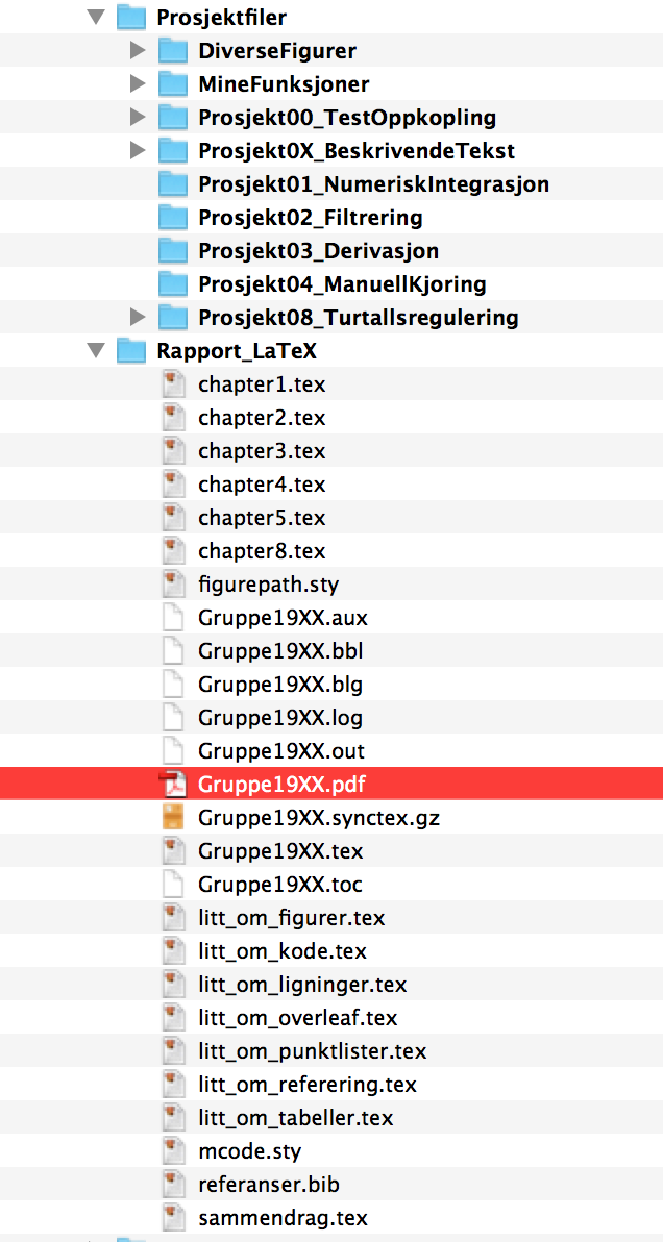
\includegraphics{mappestruktur}}
  \caption{Organisering i mappestruktur hvor {\tt DiverseFigurer}-mappen
    inneholder {\em både} figurer og undermapper med figurer, mens 
    hovedfilen ligger i {\tt Rapport\_LaTeX}-mappen. } 
  \label{fig:mappestruktur}
\end{figure}




